\begin{Pro}
   Convierte las siguientes expresiones regulares en autómatas finitos deterministas (DFA):
   \begin{enumerate}
       \item $[ab]^*$
       \item $(a?b^*)^*$
       \item $[ab]^*abb[ab]^*$
    \end{enumerate}
\end{Pro}

\begin{enumerate}
    \item $[ab]^*$

    \item $(a?b^*)^*$
    Vamos a construir primero el AFN, con el algoritmo de Thompson:
    
    \begin{figure}[ht]
        \centering
        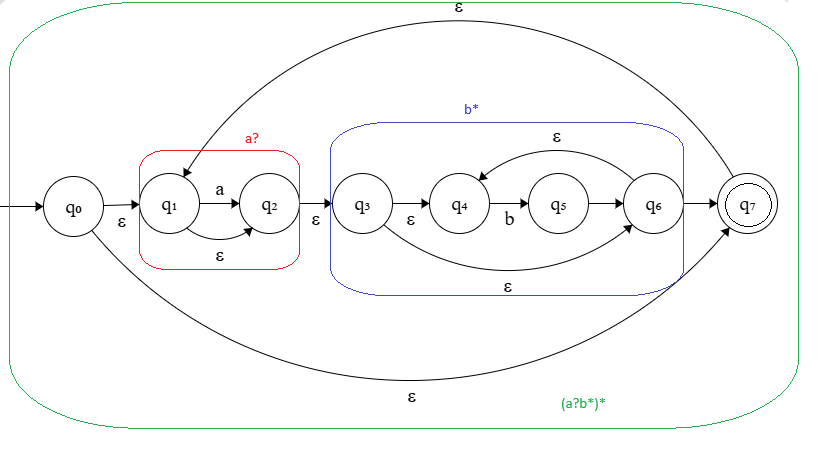
\includegraphics[width=0.5\textwidth]{images/7bAFN.png}
        \caption{Automata Finito No Determinista, ejercicio 7 b}
    \end{figure}

    Ahora vamos a convertir el AFN en un AFD, con el algoritmo de subconjuntos:
    Primero vamos a sacar las epsilon cerradura de cada estado:
    \begin{itemize}
        \item $\epsilon$-Cerradura($q_0$) = $\{q_0, q_1, q_2, q_3, q_4, q_6, q_7\}$
        \item $\epsilon$-Cerradura($q_1$) = $\{q_1, q_2, q_3, q_4, q_6, q_7\}$
        \item $\epsilon$-Cerradura($q_2$) = $\{q_1, q_2, q_3, q_4, q_6, q_7\}$
        \item $\epsilon$-Cerradura($q_3$) = $\{q_1, q_2, q_3, q_4, q_6, q_7\}$
        \item $\epsilon$-Cerradura($q_4$) = $\{q_4\}$
        \item $\epsilon$-Cerradura($q_5$) = $\{q_1, q_2, q_3, q_4, q_5, q_6, q_7\}$
        \item $\epsilon$-Cerradura($q_6$) = $\{q_1, q_2, q_3, q_4, q_6, q_7\}$
        \item $\epsilon$-Cerradura($q_7$) = $\{q_1, q_2, q_3, q_4, q_6, q_7\}$
    \end{itemize}
    Ahora vamos a construir la tabla de transiciones del AFD:
    \begin{table}[ht]        
    \centering
    \begin{tabular}{|c|c|c|}
    \hline
    \textbf{Estados} & \textbf{Transición con a} & \textbf{Transición con b } \\
    \hline
    $\epsilon$-Cerradura($q_0$) &$\epsilon$-Cerradura($q_2$) & $\epsilon$-Cerradura($q_5$) \\
    \hline      
    $\epsilon$-Cerradura($q_2$) & $\epsilon$-Cerradura($q_2$) & $\epsilon$-Cerradura($q_5$) \\
    \hline 
    $\epsilon$-Cerradura($q_5$) & $\epsilon$-Cerradura($q_5$) \\
    \hline
    \end{tabular}
    \caption{Tabla de transiciones del AFD} 
    \end{table}

    Vease que el automata queda así;

    \begin{figure}[ht]
        \centering
        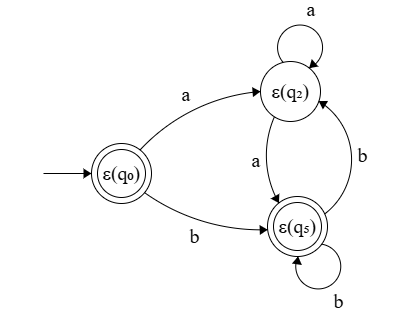
\includegraphics[width=0.5\textwidth]{images/7bDFA.png}
        \caption{Automata Finito Determinista, ejercicio 7 b}
    \end{figure}

    Sí aplicamos el algoritmo de minimización de DFA, queda de la siguiente manera:
    \begin{figure}[ht]
        \centering
        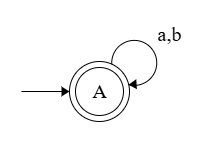
\includegraphics[width=0.5\textwidth]{images/7bDFAminimo.png}
        \caption{Automata Finito Determinista Mínimo, ejercicio 7 b}
    \end{figure}

    \item $[ab]^*abb[ab]^*$ \\
    Por el primer ejercicio sabemos que el autómata para $[ab]^*$ es:
    \begin{figure}[ht]   
        \centering
        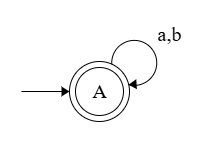
\includegraphics[width=0.5\textwidth]{images/7bDFAminimo.png}
        \caption{Automata Finito Determinista, ejercicio 7 a}
    \end{figure}
    Ahora vamos a construir el autómata para $[ab]^*abb[ab]^*$: 
    \begin{figure}[ht]
        \centering
        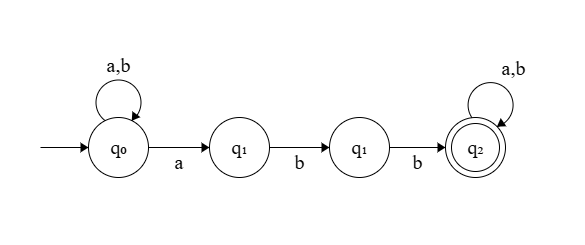
\includegraphics[width=0.5\textwidth]{images/7c.png}
        \caption{Automata Finito Determinista, ejercicio 7 c}
    \end{figure}
\end{enumerate}